\documentclass[a4paper,11pt]{article}

% Use utf-8 encoding for foreign characters
\usepackage[utf8]{inputenc}
\usepackage[british,english]{babel}
\usepackage[T1]{fontenc}

% Setup for fullpage use
\usepackage{fullpage}

% Multipart figures
\usepackage{subfigure}

% More symbols
\usepackage{amsmath}
\usepackage{amssymb}
\usepackage{latexsym}

% For pretty URLs, see: http://en.wikibooks.org/wiki/LaTeX/Hyperlinks
\usepackage{hyperref}

% Surround parts of graphics with box
\usepackage{boxedminipage}

% Package for including code in the document
\usepackage{listings}

% If you want to generate a toc for each chapter (use with book)
\usepackage{minitoc}

% Uncomment if you want to use Palatino as font
\usepackage[sc]{mathpazo}
\linespread{1.05}         % Palatino needs more leading (space between lines)

% This is now the recommended way for checking for PDFLaTeX:
\usepackage{ifpdf}


\addto\captionsenglish{\renewcommand{\refname}{}}

%\newif\ifpdf
%\ifx\pdfoutput\undefined
%\pdffalse % we are not running PDFLaTeX
%\else
%\pdfoutput=1 % we are running PDFLaTeX
%\pdftrue
%\fi

\ifpdf
\usepackage[pdftex]{graphicx}
\else
\usepackage{graphicx}
\fi
\title{Deliverable 4: Sprint \#1\\\small{for}\\\small{Danske Bank: Peer-to-peer}}
\author{ Group Delta:\\Jesper Borgstrup, Thomas Kjeldsen and Mads Ohm Larsen }

\date{April 1, 2011}

\begin{document}

\ifpdf
\DeclareGraphicsExtensions{.pdf, .jpg, .tif}
\else
\DeclareGraphicsExtensions{.eps, .jpg}
\fi

\maketitle

%\tableofcontents
%\vspace{2cm}

%%%%%%%%%%%%%%%%%%%%%%%%%%%%%%%%%%%%%%
%%%%%%%%%%%%%%%%%%%%%%%%%%%%%%%%%%%%%%
%%%%%%%%%%%%%%%%%%%%%%%%%%%%%%%%%%%%%%

\section{Requirements for this deliverable}
\begin{enumerate}
\item Doing a demo in class (on 2011-03-30)
\item Giving us access to your source code
\item Handing in a collection of your sprint material
\item Describing a sprint retrospective (e.g., as a set of bullets outlining what
when well, what went wrong, and how you will improve for the next sprint)
\end{enumerate}

The Sprint Demo was given on March 30th. This document describes requirements 2-4 as well as the sprint learning goal -- software design and architecture.

%%%%%%%%%%%%%%%%%%%%%%%%%%%%%%%%%%%%%%
%%%%%%%%%%%%%%%%%%%%%%%%%%%%%%%%%%%%%%
%%%%%%%%%%%%%%%%%%%%%%%%%%%%%%%%%%%%%%

\section{Software architecture}
Although our software currently is implemented as a standalone application, we intend, for our third sprint, to divide the functionality into two parts:
\begin{itemize}
\item An independent library responsible for establishing a secure bluetooth connection between two phones aided by an initial out-of-band (OOB) connection such as Bump.
\item A sample application utilizing the library to securely send arbitrary files (e.g. pictures, video or music) to another nearby device using the aforementioned bluetooth connection.
\end{itemize}

As such, we are using layers to separate different parts of the application.
The sample application needs not know about how the library is implemented, i.e. how it establishes a secure bluetooth connection, but can rely on that the library makes it happen and exposes an interface for doing so.

%%%%%%%%%%%%%%%%%%%%%%%%%%%%%%%%%%%%%%
%%%%%%%%%%%%%%%%%%%%%%%%%%%%%%%%%%%%%%
%%%%%%%%%%%%%%%%%%%%%%%%%%%%%%%%%%%%%%

\section{Software design}
\paragraph{Identity providers}
An OOB connection used to exchange bluetooth identity information to setup the actual connection will be known as an \emph{identity provider}. In order to seamlessly support multiple identity providers, we plan on using the Abstract Factory\cite{GangOfFour} pattern. This way, a user of the API will not have to know about or rely upon the implementations of the different identity providers, but simply decide which provider to use.

\paragraph{Android Intents}
Luckily, parts of the Android API seems to have been designed with some design patterns in mind. As such, the Android intent system seems inspired by the Command\cite{GangOfFour} pattern with which you encapsulate all the information needed the call a method when appropriate, so the system asynchronously can call the method.

%%%%%%%%%%%%%%%%%%%%%%%%%%%%%%%%%%%%%%
%%%%%%%%%%%%%%%%%%%%%%%%%%%%%%%%%%%%%%
%%%%%%%%%%%%%%%%%%%%%%%%%%%%%%%%%%%%%%

\section{Source code access}
Our source code is publicly available on Github from \url{https://github.com/omegahm/DBP2P}.

%Please note that we are working on multiple branches (use the button switch branch to view another branch).

%The master branch currently holds only documentation and deliverables, while we have a dedicated development branch for sprint \#1 named \texttt{dustytuba}.

If you wish to checkout our code (read-only) using Git, then use git clone with this URL:
\url{git://github.com/omegahm/DBP2P.git}

%%%%%%%%%%%%%%%%%%%%%%%%%%%%%%%%%%%%%%
%%%%%%%%%%%%%%%%%%%%%%%%%%%%%%%%%%%%%%
%%%%%%%%%%%%%%%%%%%%%%%%%%%%%%%%%%%%%%

\section{Sprint material}
Sprint Material needed to assess our progress include the following:
\begin{itemize}
\item source code (version number and access method is sufficient)
\item product backlog (before and after the sprint)
\item sprint backlog
\item any other material (e.g., burndown chart) that illustrates your progress
\end{itemize}


\subsection{Source Code}

The final product of sprint \#2 has been tagged \href{https://github.com/omegahm/DBP2P/tree/sprintdemo2}{\tt sprintdemo2}. in the git repository, where the application is located in the folder {\tt DustyTubaSampleApp}.

The following main tasks have been completed during this sprint:
\begin{itemize}
	\item Establish Bluetooth connection (2.1+ devices only)
	\item Send and receive file through the bluetooth connection (to be sample app) (backlog from sprint 2)
\end{itemize}

In regards to our user stories, the tasks completed correspond to the following user stories:
\begin{verbatim}
  As a        user
  I want to   be able to easily setup a local, secure connection between two Android phones
  Such that   no 3rd party can read or alter the communication

  As a        user
  I want to   transfer any item I have selected on my device to a nearby device
  Such that   I can easily transfer said item
\end{verbatim}

The second story, though, has not been completed for ``any item'', but only for web pages and images so far. The remainder has been moved to the forthcoming sprint 3.

\subsection{Product Backlog}
Our sprint backlog is shown in figure \ref{productbacklog} on page \pageref{productbacklog}.

\begin{figure}[ht!]
	\begin{center}
	% Insert sprint backlog here
	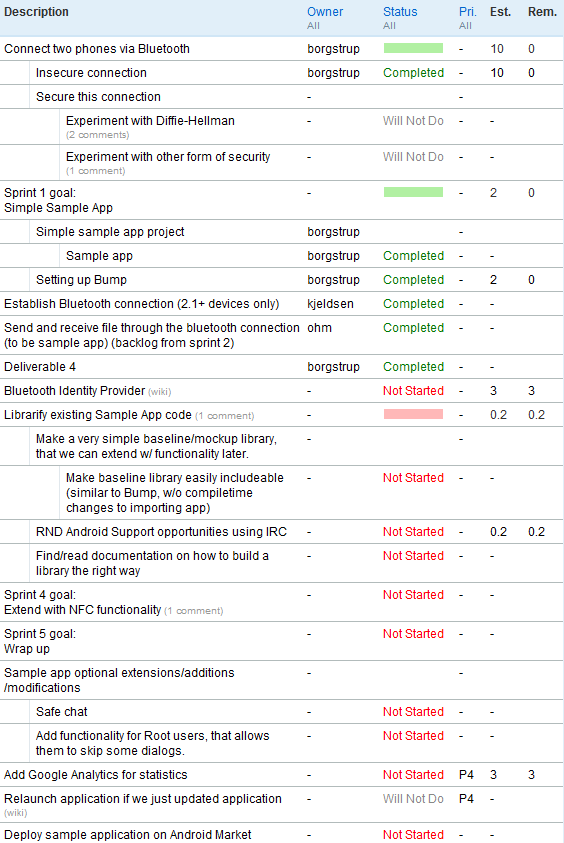
\includegraphics[width=0.9\textwidth]{productbacklog.png}		
	\end{center}
	\caption{Our product backlog at the end of sprint \#2.}
	\label{productbacklog}
\end{figure}

\subsection{Sprint Backlog}
Our sprint backlog is shown in figure \ref{sprintbacklog} on page \pageref{sprintbacklog}.

\begin{figure}[ht!]
	\begin{center}
	% Insert sprint backlog here
	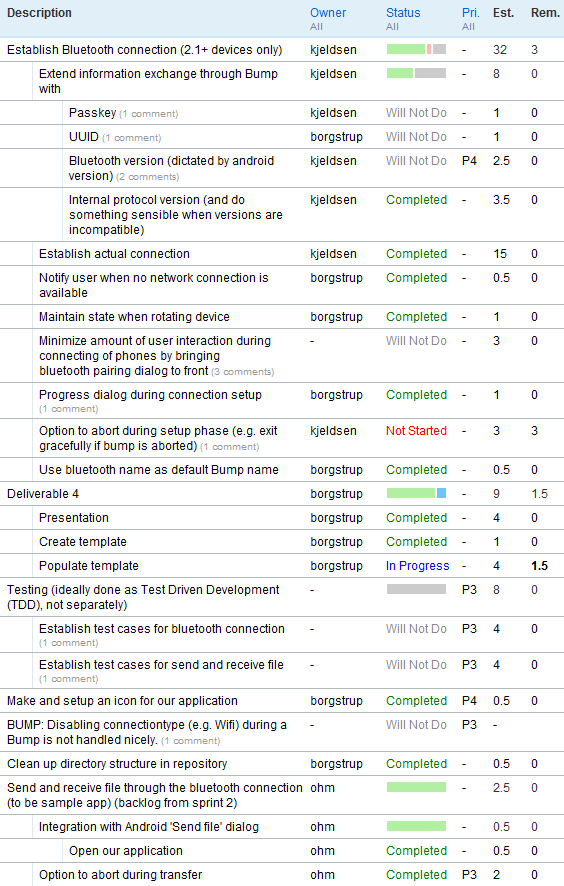
\includegraphics[width=0.85\textwidth]{sprintbacklog.png}		
	\end{center}
	\caption{Our sprint backlog after the sprint was finished}
	\label{sprintbacklog}
\end{figure}

\subsection{Burndown chart}

Our burndown chart is shown in figure \ref{burndown} on page \pageref{burndown}.

\begin{figure}[ht!]
	\begin{center}
	% Insert burndown chart here
	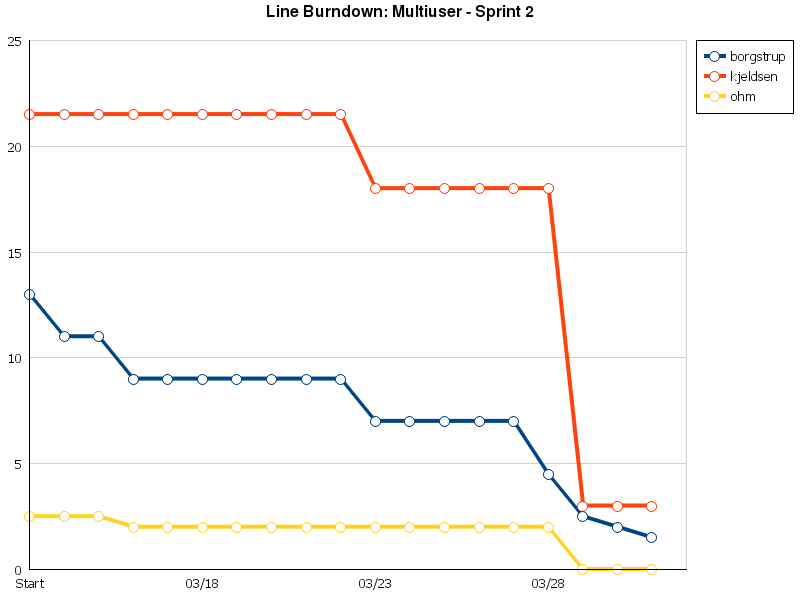
\includegraphics[width=\textwidth]{burndown.png}		
	\end{center}
	\caption{Our burndown chart at the end of the sprint}
	\label{burndown}
\end{figure}

\subsection{Other relevant material}
We have got an Acunote account\footnote{\url{http://dbp2p.acunote.com/}} setup, and access to this have been granted.

\clearpage

%%%%%%%%%%%%%%%%%%%%%%%%%%%%%%%%%%%%%%
%%%%%%%%%%%%%%%%%%%%%%%%%%%%%%%%%%%%%%
%%%%%%%%%%%%%%%%%%%%%%%%%%%%%%%%%%%%%%

\section{Sprint retrospective}

What went well during this sprint:

\begin{itemize}
	\item Better breakdown of the user stories for the sprint
	\item Collaboration through git works more smoothly
\end{itemize}

\noindent
What went wrong:

\begin{itemize}
	\item Lack of time due to heavy workload in other course
	\item Not enough virtual scrum meetings held
	\item Postponed too much work until late in the sprint
	\item For major tasks, we didn’t know when they were complete
	\item Some time estimates were overly optimistic
	\item Lack of phones (no emulator support for Bluetooth)
\end{itemize}

\noindent
How we will improve:
\begin{itemize}
	\item New scrum master will keep track of remaining workload and activate the team
	\item We will define accept criteria for major tasks
	\item We will be more conservative on time estimates for tasks
	\item We will look at the projected burndown and react faster rather than an all-in end-of-sprint.
\end{itemize}

\section{References}
\begin{thebibliography}{9}
\vspace{-3em}

\bibitem{GangOfFour}
  Gamma et al.,
  \emph{Design Patterns: Elements of Reusable Object-Oriented Software}.
  Addison Wesley, 1994.

\end{thebibliography}

\end{document}
